\documentclass{article}

\usepackage[T1]{fontenc}
\usepackage{textcomp}

\usepackage[english]{babel}
\usepackage[utf8]{inputenc}

\usepackage{lmodern}

\usepackage{hyperref}
\hypersetup{breaklinks}
\hypersetup{pdfborder=0 0 0}

\usepackage{datetime}
\newdateformat{jpmdate}{\THEDAY~\monthname[\THEMONTH] \THEYEAR}
\AtBeginDocument{\jpmdate}

\usepackage[babel=true]{microtype}

\usepackage{amsmath}

\usepackage{geometry}

\usepackage{tikz}

\usepackage[normalem]{ulem}


\title{The impact of vector interaction with other insect species on
  disease spread}

\author{
  Elizabeth Borer
  \and
  David Crowder
  \and
  Deborah Finke
  \and
  Jing Li
  \and
  Jan Medlock
  \and
  David Pattemore
  \and
  Rakefet Sharon
}


\newcommand{\md}{\mathrm{d}}
\newcommand{\me}{\mathrm{e}}
\newcommand{\mT}{\mathrm{T}}
\newcommand{\mat}[1]{\mathbf{#1}}
\renewcommand{\vec}[1]{\mathbf{#1}}
\newcommand{\elasticity}[2]{\mathcal{E}_{#2}\negthickspace\left({#1}\right)}


\begin{document}

\maketitle

\textbf{Does the model have the gamma-distributed infection time that
  we want?}


\section{Model description}


\subsection{Movement \& feeding model}

Initially, vectors are moving: the number of moving vectors is
$V_M(t)$.  After an exponential waiting time with mean duration
$1 / \sigma_V$, they begin feeding on a plant: the number of feeding
vectors is $V_F(t)$.  They stop feeding and go back to the moving
state after an exponential waiting time of $1 / \tau_V$.  Including
birth and death, the numbers over time evolve by
\begin{equation}
  \begin{split}
    \frac{\md V_M}{\md t} &=
    - \sigma_V V_M + \tau_V V_F - \mu_V V_M
    + b_V V \left[1 - \frac{V(t)}{K_V}\right],
    \\
    \frac{\md V_F}{\md t} &=
    \sigma_V V_M - \tau_V V_F - \mu_V V_F,
  \end{split}
\end{equation}
where $V = V_F + V_M$.

Dropping birth and death, the probability density for the time between
the start of one feeding to the start of the next feeding is $V_G(t)$
that satisfies
\begin{equation}
  \begin{aligned}
    \frac{\md V_F}{\md t} &=
    - \tau_V V_F,
    & V_F(0) &= 1,
    \\
    \frac{\md V_M}{\md t} &=
    \tau_V V_F - \sigma_V V_M,
    & V_M(0) &= 0,
    \\
    \frac{\md V_G}{\md t} &=
    \sigma_V V_M,
    & V_G(0) &= 0,
  \end{aligned}
\end{equation}
which is
\begin{equation}
  \begin{split}
    V_F(t) &= \me^{-\tau_V t},
    \\
    V_M(t) &= \frac{\tau_V}{\tau_V - \sigma_V}
    \me^{- \sigma_V t} \left(
      1 - \me^{- (\tau_V -\sigma_V) t}
    \right)
    = \frac{\tau_V}{\sigma_V - \tau_V}
    \me^{- \tau_V t} \left(
      1 - \me^{- (\sigma_V - \tau_V) t}
    \right),
    \\
    V_G(t) &= 1
    - \frac{\tau_V}{\tau_V - \sigma_V} \me^{- \sigma_V t}
    + \frac{\sigma_V}{\tau_V - \sigma_V} \me^{- \tau_V t},
  \end{split}
\end{equation}



\subsection{Full model}

Let $r$ be the level of interaction of the vector species with the
other insect species, with $r = 0$ being no interaction.  Initially,
we will consider just this implicit representation of the 2nd insect
species, but later we will explicitly model this population as well.

Let $V_{MS}(t)$ and $V_{FS}(t)$ be the number of moving and feeding
susceptible vectors at time $t$ and $V_{MI}(t)$ and $V_{FI}(t)$ be the
number of moving and feeding infectious vectors at time $t$.
Likewise, let $P_S(t)$ and $P_I(t)$ be the number of susceptible and
infective plants at time $t$.  The total number of vectors is
$V(t) = V_{MS}(t) + V_{FS}(t) + V_{MI}(t) + V_{FI}(t)$ and the total
number of plants is $P(t) = P_S(t) + P_I(t)$.  The model is
\begin{equation}
  \label{odesystemdimensional}
  \begin{split}
    \frac{\md V_{MS}}{\md t}(t)
    &=
    - \tau_V V_{MS}(t)
    + \sigma_V V_{FS}(t)
    + \gamma_V V_{MI}(t)
    - \mu_V V_{MS}(t)
    + b_V V(t) \left[1 - \frac{V(t)}{K_V}\right],
    \\
    \frac{\md V_{FS}}{\md t}(t)
    &= - \beta_V \frac{P_I(t)}{P(t)} V_{FS}(t)
    + \tau_V V_{MS}(t)
    - \sigma_V V_{FS}(t)
    + \gamma_V V_{FI}(t)
    - \mu_V V_{FS}(t),
    \\
    \frac{\md V_{MI}}{\md t}(t)
    &=
    - \tau_V V_{MI}(t)
    + \sigma_V V_{FI}(t)
    - \gamma_V V_{MI}(t)
    - \mu_V V_{MI}(t),
    \\
    \frac{\md V_{FI}}{\md t}(t)
    &=
    \beta_V \frac{P_I(t)}{P(t)} V_{FS}(t)
    + \tau_V V_{MI}(t)
    - \sigma_V V_{FI}(t)
    - \gamma_V V_{FI}(t)
    - \mu_V V_{FI}(t),
    \\
    \frac{\md P_S}{\md t}(t)
    &= - \beta_P V_{FI}(t) \frac{P_S(t)}{P(t)}
    - \mu_P P_S(t)
    + b_P P(t) \left[1 - \frac{P(t)}{K_P}\right],
    \\
    \frac{\md P_I}{\md t}(t)
    &= \beta_P V_{FI}(t) \frac{P_S(t)}{P(t)}
    - \mu_P P_I(t),
  \end{split}
\end{equation}
where $\beta_V$ is the infection rate from plants to vectors,
$\beta_P$ is the infection rate from vectors to plants, $\gamma_V$ is
the rate of pathogen clearance in vectors, $\mu_V$ is the death rate
of vectors, $\mu_P$ is the death rate of vectors, $b_V$ is the birth
rate of vectors in the absence of crowding, $b_P$ is the birth rate of
vectors in the absence of crowding, $K_V$ is the carrying capacity of
vectors and $K_P$ is the carrying capacity of vectors (n.b.~this is
the population density at which birth rate is $0$, not where the birth
rate is equal to the death rate).

\begin{figure}
  \centering
  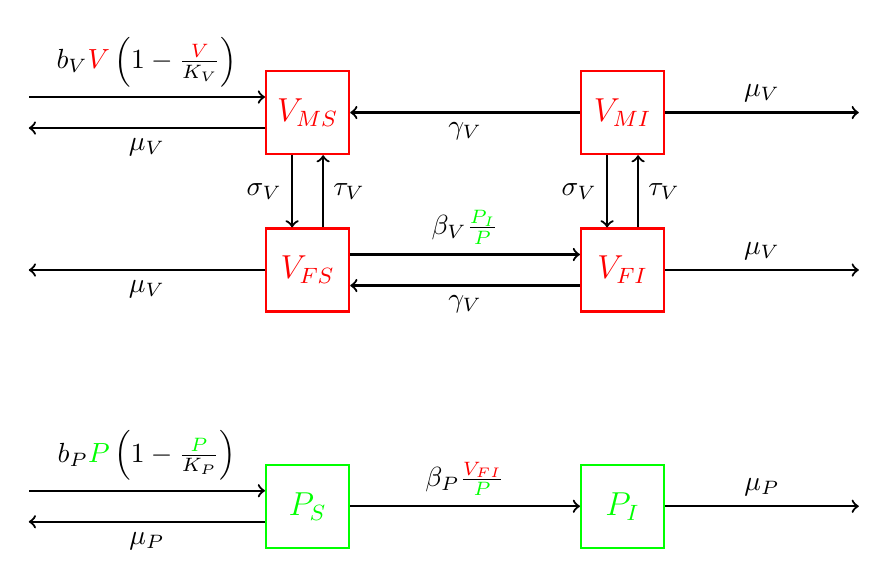
\begin{tikzpicture}[
    thick,
    scale = 1,
    %
    compartment/.style = {draw,
      font = \large,
      minimum size = {3em}},
    %
    plant/.style = {green},
    vector/.style = {red},
    ]

    \node at (0, 5)
    [compartment, vector, name = V_MS] {$V_{MS}$};
    \node at (4, 5)
    [compartment, vector, name = V_MI] {$V_{MI}$};

    \node at (0, 3)
    [compartment, vector, name = V_FS] {$V_{FS}$};
    \node at (4, 3)
    [compartment, vector, name = V_FI] {$V_{FI}$};

    \node at (0, 0)
    [compartment, plant, name = P_S] {$P_S$};
    \node at (4, 0)
    [compartment, plant, name = P_I] {$P_I$};

    \draw [->] (P_S) to node [above]
    {$\beta_P \frac{\textcolor{red}{V_{FI}}}{\textcolor{green}{P}}$}
    (P_I);

    \draw [->] (V_FS.20) to node [above]
    {$\beta_V \frac{\textcolor{green}{P_I}}{\textcolor{green}{P}}$}
    (V_FI.160);

    \draw [->] (V_FI.200) to node [below] {$\gamma_V$} (V_FS.340);
    \draw [->] (V_MI) to node [below] {$\gamma_V$} (V_MS);

    \draw [->] (V_MS.250) to node [left] {$\sigma_V$} (V_FS.110);
    \draw [->] (V_MI.250) to node [left] {$\sigma_V$} (V_FI.110);

    \draw [->] (V_FS.70) to node [right] {$\tau_V$} (V_MS.290);
    \draw [->] (V_FI.70) to node [right] {$\tau_V$} (V_MI.290);

    \draw [<-] (P_S.160) to node [above]
    {$b_P \textcolor{green}{P} \left(1 - \frac{\textcolor{green}{P}}{K_P}\right)$}
    +(180: 3);

    \draw [->] (P_S.200) to node [below] {$\mu_P$} +(180: 3);

    \draw [->] (P_I) to node [above] {$\mu_P$} +(0: 3);

    \draw [<-] (V_MS.160) to node [above]
    {$b_V \textcolor{red}{V} \left(1 - \frac{\textcolor{red}{V}}{K_V}\right)$}
    +(180: 3);

    \draw [->] (V_FS.180) to node [below] {$\mu_V$} +(180: 3);
    \draw [->] (V_MS.200) to node [below] {$\mu_V$} +(180: 3);

    \draw [->] (V_FI) to node [above] {$\mu_V$} +(0: 3);
    \draw [->] (V_MI) to node [above] {$\mu_V$} +(0: 3);

  \end{tikzpicture}
  \caption{Model diagram.  $P_S$ and $P_I$ (green) are the numbers
    of uninfected and plants.  $V_S$ and $V_I$ (red) are numbers of
    uninfected and infected vectors.}
\end{figure}


\section{Nondimensionalization}

The disease-free steady state is
\begin{align}
  V^* &= K_V \left(1 - \frac{\mu_V}{b_V}\right),
  &
  V_{MS} &= \frac{\tau_V + \mu_V}{\sigma_V + \tau_V + \mu_V} V^*,
  &
  V_{FS} &= \frac{\sigma_V}{\sigma_V + \tau_V + \mu_V} V^*,
  \\
  P^* &= P_V \left(1 - \frac{\mu_P}{b_P}\right),
  &
  P_S &= P^*,
  \\
  V_{MI} &= 0,
  &
  V_{FI} &= 0,
  &
  P_I &= 0.
\end{align}
We will use $V^*$ for the scale of $V_{MS}$, $V_{FS}$, $V_{MI}$ and
$V_{FI}$; $P^*$ for the scale of $P_S$ and $P_I$; and $\beta_V$ for
the time scale:
\begin{equation}
  \begin{aligned}
    \hat{V}_{MS} &= \frac{V_{MS}}{V^*},
    &
    \hat{V}_{FS} &= \frac{V_{FS}}{V^*},
    &
    \hat{V}_{MI} &= \frac{V_{MI}}{V^*},
    &
    \hat{V}_{FI} &= \frac{V_{FI}}{V^*},
    \\
    \hat{P}_S &= \frac{P_S}{P^*},
    &
    \hat{P}_I &= \frac{P_I}{P^*},
    &
    \hat{t} &= \beta_V t,
    \\
    \hat{\beta}_P &= \frac{\beta_P}{\beta_V},
    &
    \hat{\gamma}_V &= \frac{\gamma_V}{\beta_V},
    &
    \hat{b}_V &= \frac{b_V}{\beta_V},
    &
    \hat{\mu}_V &= \frac{\mu_V}{\beta_V},
    \\
    \hat{\sigma}_V &= \frac{\sigma_V}{\beta_V},
    &
    \hat{\tau}_V &= \frac{\tau_V}{\beta_V},
    &
    \hat{b}_P &= \frac{b_P}{\beta_V},
    &
    \hat{\mu}_P &= \frac{\mu_P}{\beta_V},
  \end{aligned}
\end{equation}
Then
\begin{equation}
  \label{odesystem}
  \begin{split}
    \frac{\md \hat{V}_{MS}}{\md \hat{t}}
    &=
    - \hat{\tau}_V \hat{V}_{MS}
    + \hat{\sigma}_V \hat{V}_{FS}
    + \hat{\gamma}_V \hat{V}_{MI}
    - \hat{\mu}_V \hat{V}_{MS}
    + \hat{b}_V \hat{V} \left[
      1 - \left(1 - \frac{\hat{\mu}_V}{\hat{b}_V}\right)
      \hat{V}
    \right],
    \\
    \frac{\md \hat{V}_{FS}}{\md \hat{t}}
    &= - \frac{\hat{P}_I}{\hat{P}} \hat{V}_{FS}
    + \hat{\tau}_V \hat{V}_{MS}
    - \hat{\sigma}_V \hat{V}_{FS}
    + \hat{\gamma}_V \hat{V}_{FI}
    - \hat{\mu}_V \hat{V}_{FS},
    \\
    \frac{\md \hat{V}_{MI}}{\md \hat{t}}
    &=
    - \hat{\tau}_V \hat{V}_{MI}
    + \hat{\sigma}_V \hat{V}_{FI}
    - \hat{\gamma}_V \hat{V}_{MI}
    - \hat{\mu}_V \hat{V}_{MI},
    \\
    \frac{\md \hat{V}_{FI}}{\md \hat{t}}
    &=
    \frac{\hat{P}_I}{\hat{P}} \hat{V}_{FS}
    + \hat{\tau}_V \hat{V}_{MI}
    - \hat{\sigma}_V \hat{V}_{FI}
    - \hat{\gamma}_V \hat{V}_{FI}
    - \hat{\mu}_V \hat{V}_{FI},
    \\
    \frac{\md \hat{P}_S}{\md \hat{t}}
    &= - \hat{\beta}_P \hat{V}_{FI} \frac{\hat{P}_S}{\hat{P}}
    - \hat{\mu}_P \hat{P}_S
    + \hat{b}_P \hat{P}
    \left[
      1 - \left(1 - \frac{\hat{\mu}_V}{\hat{b}_V}\right) \hat{P}
    \right],
    \\
    \frac{\md \hat{P}_I}{\md t}
    &= \hat{\beta}_P \hat{V}_{FI} \frac{\hat{P}_S}{\hat{P}}
    - \hat{\mu}_P \hat{P}_I.
  \end{split}
\end{equation}
In what follows, we will drop the $\hat{}$, which hopefully won't
cause too much confusion.

\section{$R_0$ analysis}

The infected states are
\begin{equation}
  \vec{u} =
  \begin{pmatrix}
    V_{MI} \\ V_{FI} \\ P_I
  \end{pmatrix}.
\end{equation}
System \eqref{odesystem} can be written as
\begin{equation}
  \frac{\md \vec{u}}{\md t} =
  \mathcal{F}(\vec{u})
  - \mathcal{V}(\vec{u}),
\end{equation}
with infection rates
\begin{equation}
  \label{scriptF}
  \mathcal{F} =
  \begin{pmatrix}
    0
    \\
    \frac{P_I}{P} V_{FS}
    \\
    \beta_P V_{FI} \frac{P_S}{P}
  \end{pmatrix}
\end{equation}
and the remaining rates
\begin{equation}
  \label{scriptV}
  \mathcal{V} =
  \begin{pmatrix}
    \tau_V V_{MI} - \sigma_V V_{FI} + \gamma_V V_{MI} + \mu_V V_{MI}
    \\
    - \tau_V V_{MI} + \sigma_V V_{FI} + \gamma_V V_{FI} + \mu_V V_{FI}
    \\
    \mu_P P_I
  \end{pmatrix}.
\end{equation}

The disease-free equilibrium has the susceptible vectors and plants at
their carrying capacities and no infectious vectors or plants,
\begin{align}
  V_{MS} &= \frac{\sigma_V + \mu_V}{\tau_V + \sigma_V + \mu_V},
  &
  V_{FS} &= \frac{\tau_V}{\tau_V + \sigma_V + \mu_V},
  &
  V_{MI} &= 0,
  &
  V_{FI} &= 0,
  \\
  P_S &= 1,
  &
  P_I &= 0.
\end{align}
Linearizing
\eqref{scriptF} and \eqref{scriptV} at the disease-free equilibrium
gives
\begin{equation}
  \begin{split}
    \mat{F} &=
    \begin{bmatrix}
      0 & 0 & 0
      \\
      0 & 0 & \frac{\tau_V}{\tau_V + \sigma_V + \mu_V}
      \\
      0 & \beta_P & 0
    \end{bmatrix},
    \\
    \mat{V} &=
    \begin{bmatrix}
      \tau_V + \gamma_V + \mu_V & - \sigma_V & 0
      \\
      - \tau_V & \sigma_V + \gamma_V + \mu_V & 0
      \\
      0 & 0 & \mu_P
    \end{bmatrix}.
  \end{split}
\end{equation}
The residence times are
\begin{equation}
  \mat{V}^{-1} =
  \begin{bmatrix}
    \frac{\sigma_V + \gamma_V + \mu_V}
    {(\gamma_V + \mu_V) (\sigma_V + \tau_V + \mu_V + \gamma_V)}
    &  \frac{\sigma_V}
    {(\gamma_V + \mu_V) (\sigma_V + \tau_V + \mu_V + \gamma_V)}
    & 0
    \\
    \frac{\tau_V}
    {(\gamma_V + \mu_V) (\sigma_V + \tau_V + \mu_V + \gamma_V)}
    & \frac{\tau_V + \gamma_V + \mu_V}
    {(\gamma_V + \mu_V) (\sigma_V + \tau_V + \mu_V + \gamma_V)}
    & 0
    \\
    0 & 0 & \frac{1}{\mu_P}
  \end{bmatrix}.
\end{equation}
Then the next-generation matrix is
\begin{equation}
  \begin{split}
    \mat{G} &= \mat{F} \mat{V}^{-1}
    \\
    &=
    \begin{bmatrix}
      0 & 0 & 0
      \\
      0 & 0 & \frac{\tau_V}{\mu_P (\tau_V + \sigma_V + \mu_V)}
      \\
      \frac{\beta_P \tau_V}
      {(\gamma_V + \mu_V) (\sigma_V + \tau_V + \mu_V + \gamma_V)}
      & \frac{\beta_P (\tau_V + \gamma_V + \mu_V)}
      {(\gamma_V + \mu_V) (\sigma_V + \tau_V + \mu_V + \gamma_V)}
      & 0
    \end{bmatrix}.
  \end{split}
\end{equation}
The leading eigenvalue of $G$ is
\begin{equation}
  R_0 = \sqrt{
    \frac{\beta_P \tau_V}
    {\mu_P (\gamma_V + \mu_V) (\sigma_V + \tau_V + \mu_V + \gamma_V)}
  }
\end{equation}
or
\begin{equation}
  R_0^2 =
  \frac{\beta_P \tau_V}
  {\mu_P (\gamma_V + \mu_V) (\sigma_V + \tau_V + \mu_V + \gamma_V)}.
\end{equation}

In dimensional parameters, $R_0$ is
\begin{equation}
  R_0^2 =
  \frac{\beta_P \beta_V \tau_V}
  {\mu_P \left(\gamma_V + \mu_V\right)
    \left(\sigma_V + \tau_V + \gamma_V + \mu_V\right)},
\end{equation}
or
\begin{equation}
  R_0^2 =
  \beta_V \frac{1}{\mu_P}
  \beta_P
  \frac{1}{\gamma_V + \mu_V}
  \frac{\tau_V}
  {\sigma_V + \tau_V + \gamma_V + \mu_V},
\end{equation}
where $\beta_V$ is the transmission rate from infected plants to
susceptible vectors, $\frac{1}{\mu_P}$ is the duration of
infectiousness in plants, $\beta_P$ is the transmission rate from
infected vectors to susceptible plants, $\frac{1}{\gamma_V + \mu_V}$
is the duration of infectiousness in vectors, and
$\frac{\tau_V}{\sigma_V + \tau_V + \gamma_V + \mu_V}$ is the
proportion of the vectors' infectious period spent feeding.


\section{Increasing $n$}

We are initially thinking that the effects of the second insect
species will only be on vector death rate and vector movement rate,
and for now we will take these to have constant semi-elasticity for
simplicity:
\begin{equation}
  \begin{split}
    \mu_V(n) &= \overline{\mu_V} \me^{\epsilon_{\mu_V} n},
    \\
    \tau_V(n) &= \overline{\tau_V} \me^{\epsilon_{\tau_V} n}.
  \end{split}
\end{equation}

Then
\begin{equation}
  \begin{split}
    \elasticity{R_0^2}{n} &=
    \frac{1}{R_0^2} \frac{\md R_0^2}{\md n}
    \\
    &=
    \frac{\left(\gamma_V + \mu_V\right)
      \left(\sigma_V + \tau_V + \gamma_V + \mu_V\right)}
    {\tau_V}
    \frac{\md}{\md n}
    \left(
      \frac{1}{\gamma_V + \mu_V}
      \frac{\tau_V}{\sigma_V + \tau_V + \gamma_V + \mu_V}
    \right)
    \\
    &=
    \frac{\left(\gamma_V + \mu_V\right)
      \left(\sigma_V + \tau_V + \gamma_V + \mu_V\right)}
    {\tau_V}
    \frac{\partial}{\partial \mu_V}
    \left(
      \frac{1}{\gamma_V + \mu_V}
      \frac{\tau_V}{\sigma_V + \tau_V + \gamma_V + \mu_V}
    \right)
    \frac{\md \mu_V}{\md n}
    \\ & \quad\quad\quad {}
    + \frac{\left(\gamma_V + \mu_V\right)
      \left(\sigma_V + \tau_V + \gamma_V + \mu_V\right)}
    {\tau_V}
    \frac{1}{\gamma_V + \mu_V}
    \frac{\partial}{\partial \tau_V}
    \left(
      \frac{\tau_V}{\sigma_V + \tau_V + \gamma_V + \mu_V}
    \right)
    \frac{\md \tau_V}{\md n}
    \\
    &=
    - \left(
      \frac{1}{\gamma_V + \mu_V}
      +
      \frac{1}{\sigma_V + \tau_V + \gamma_V + \mu_V}
    \right)
    \mu_V \epsilon_{\mu_V}
    +
    \frac{\sigma_V + \gamma_V + \mu_V}
    {\sigma_V + \tau_V + \gamma_V + \mu_V}
    \epsilon_{\tau_V}.
  \end{split}
\end{equation}


\section{Plots to make}

\begin{itemize}
\item Persistent vs.~non-persistent
\item Movement, birth, death
\item Number of interactors
\end{itemize}

\begin{itemize}
\item $R_0$ vs.~$n$
\item $R_0$ (or $\md R_0$) vs.~$\epsilon$'s (imshow, pcolor, contour,
  etc)
\item How to balance results from sensitivities (i.e.~derivatives)
  vs.~results from choosing functional forms.
\end{itemize}

\end{document}
